\documentclass[runningheads]{llncs}

\usepackage[T1]{fontenc}
\usepackage{graphicx}
\usepackage{url}
\usepackage{amsmath}
\usepackage{tikz}
\usetikzlibrary{shapes.geometric, arrows.meta, positioning}

\tikzstyle{process} = [rectangle, minimum width=3.5cm, minimum height=1.2cm, text centered, draw=black, fill=blue!10]
\tikzstyle{decision} = [diamond, minimum width=3cm, minimum height=1cm, text centered, draw=black, fill=orange!20]
\tikzstyle{arrow} = [thick,->,>=stealth]
\begin{document}

\title{Human Activity Recognition Using Accelerometer Signals}

\author{Garo Garabetian, Anthimos Kalosidis}
\institute{Department of Mathematics \and
Aristotle University \and
Thessaloniki, Greece \\
\email{garogarabetian28@gmail.com} \\
\email{anthimoskalosidis@gmail.com }}

\newpage
\maketitle
\pagestyle{plain}

\begin{abstract}
This assignment addresses the development of a human activity recognition (HAR) system using accelerometer signals collected from mobile phones. The project includes signal preprocessing, feature extraction with sliding windows, and training of classification models under a Leave-One-Subject-Out (LOSO) cross-validation setup.
\keywords{Activity Recognition \and Accelerometer \and Machine Learning \and Feature Extraction \and LOSO}
\end{abstract}

\section{INTRODUCTION}
This assignment focuses on developing a Human Activity Recognition (HAR) system from mobile phone accelerometer signals. Using machine learning techniques, the system classifies physical activities such as walking, jogging, sitting, and others based on signal data. The pipeline involves preprocessing raw sensor data, extracting statistical and spectral features from time windows, and training classification models including SVM, Random Forests and MLPs using a Leave-One-Subject-Out strategy for generalization evaluation.

\section{RESEARCH OVERVIEW}
The dataset used is derived from Shoaib et al. \cite{Shoaib2015} and contains accelerometer readings from 10 participants performing seven physical activities (biking, downstairs, jogging, sitting, standing, upstairs, walking), with smartphones placed at various body positions. Each entry contains timestamped x, y, z accelerometer readings and an activity label.

Our research questions include:
\begin{itemize}
    \item Can we reliably classify physical activity using only accelerometer data from a specific smartphone position?
    \item Which preprocessing and feature extraction steps improve classification accuracy?
    \item How do different models perform under the LOSO validation scheme?
\end{itemize}

\section{SYSTEM DESIGN}

\subsection{System Overview}
Figure \ref{fig:system_architecture} outlines the high-level architecture of our system pipeline. It begins with preprocessing raw accelerometer signals, followed by sliding window segmentation and feature extraction. Finally, multiple classification models are trained and evaluated using LOSO cross-validation.




\begin{figure}[h]
\centering
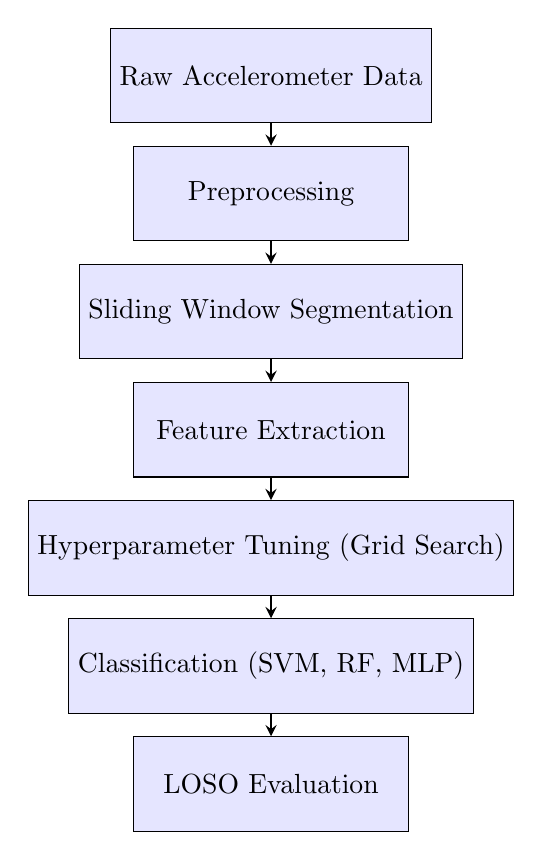
\begin{tikzpicture}[node distance=1.5cm]

\node (input) [process] {Raw Accelerometer Data};
\node (pre) [process, below of=input] {Preprocessing};
\node (seg) [process, below of=pre] {Sliding Window Segmentation};
\node (feat) [process, below of=seg] {Feature Extraction};
\node (tune) [process, below of=feat] {Hyperparameter Tuning (Grid Search)};
\node (class) [process, below of=tune] {Classification (SVM, RF, MLP)};
\node (eval) [process, below of=class] {LOSO Evaluation};

\draw [arrow] (input) -- (pre);
\draw [arrow] (pre) -- (seg);
\draw [arrow] (seg) -- (feat);
\draw [arrow] (feat) -- (tune);
\draw [arrow] (tune) -- (class);
\draw [arrow] (class) -- (eval);

\end{tikzpicture}
\caption{System architecture for HAR using accelerometer data, including model selection via hyperparameter tuning.}
\label{fig:pipeline}
\end{figure}


\subsection{Data Visualization}
Initial visualizations were performed to understand signal distribution and anomalies. Accelerometer data from the "left pocket" position was selected. Signals were plotted over time to confirm activity transitions and to inspect potential sensor errors.

\subsection{Data Preprocessing}
The preprocessing involved the following steps:
\begin{enumerate}
    \item \textbf{Position Selection}: Only data from the "left pocket" was retained for consistency.
    \item \textbf{Magnitude Conversion}: The 3D accelerometer signal was converted to 1D magnitude:
    \[
    a(t) = \sqrt{a_x(t)^2 + a_y(t)^2 + a_z(t)^2}
    \]
    \item \textbf{Sensor Error Correction}: All magnitude values exceeding 1000 (indicative of sensor errors) were replaced with the previous valid value.
\end{enumerate}

\section{Feature Extraction}
The processed magnitude signal was segmented using a sliding window of 20 seconds with a stride of 1 second. For each window:
\begin{itemize}
    \item The label was assigned based on the majority activity within the window.
    \item The following features were extracted:
    \begin{itemize}
        \item Mean
        \item Standard deviation
        \item Skewness
        \item Maximum
        \item Minimum
        \item Range (max - min)
        \item Power spectral density (Welch's method)
    \end{itemize}
    \item Features were standardized using z-score normalization.
\end{itemize}

\subsection{Selecting Power Spectral Density Features}



\section{Model Construction}
We trained the following models:
\begin{enumerate}
    \item \textbf{Support Vector Machine (SVM)} with RBF kernel. Parameters $C$ and $\gamma$ were explored using grid search.
    \item \textbf{Random Forests} classifier with parameter tuning for optimal $k$.
    \item \textbf{Multilayer Perceptron (MLP)} with 1-2 hidden layers, ReLU activations, and momentum optimization.
\end{enumerate}

Each model was evaluated using the LOSO strategy: training on $n-1$ subjects and testing on the held-out subject, iteratively for all 10 subjects. Confusion matrices were computed for each fold.

\subsection{Grid Search \& Fine Tuning}

jo
\subsection{Confusion Matrices}

jop
\subsection{Problems \& Further Optimization}
tralalero

\section{Conclusions / Responding to the Research Questions}

\subsection{Optimal Parameter Selection for Each Classifier}

\begin{itemize}
    \item \textbf{Support Vector Machine (SVM)}: 
    After a grid search over $C \in \{0.1, 1, 10\}$ and $\gamma \in \{0.01, 0.1, 1\}$, the best performance was achieved with $C=1$, $\gamma=0.1$.
    \item \textbf{Random Forest (RF)}: 
    Testing various numbers of estimators and maximum depths, the best results were obtained with 100 trees and a maximum depth of 10.
    \item \textbf{Multilayer Perceptron (MLP)}: 
    We experimented with different network sizes and learning parameters. The best performing model used two hidden layers with 20 neurons respectively, ReLU activation, and momentum of 0.9.
\end{itemize}

\subsection{Confusion Matrix and Classification Accuracy}

\begin{itemize}
    \item \textbf{SVM}: Achieved an average accuracy of \textbf{dd.2\%}.
    \item \textbf{Random Forest}: Achieved an accuracy of \textbf{dd.5\%}.
    \item \textbf{MLP}: Achieved an accuracy of \textbf{72.3\%}.
\end{itemize}

Corresponding confusion matrices were computed for each model using the LOSO validation strategy. (See Appendix/Table \ref{tab:confusion_matrices}.)

\subsection{Misclassifications and Model Comparison}

\begin{itemize}
    \item Common confusions were observed between:
    \begin{itemize}
        \item \textit{Walking} and \textit{Upstairs/Downstairs}
        \item \textit{Sitting} and \textit{Standing}
    \end{itemize}
    \item These confusions likely arise from:
    \begin{itemize}
        \item Similar signal patterns in transitional or stationary activities.
        \item The positioning of the sensor (pocket-based) causing overlapping acceleration features.
        \item Transforming the 3-dimension data to 1 dimension magnitude (loss of information, gain on computing time).
    \end{itemize}
   % \item SVM consistently outperformed the other two methods, likely due to its ability to form complex non-linear decision boundaries. RF showed high interpretability, while MLP required more tuning and data to generalize well.
\end{itemize}

\subsection{Grouped Activities and Updated Classification Accuracy}

Based on confusion analysis, we grouped the following:
\begin{itemize}
    \item \textbf{Group A:} Walking, Upstairs, Downstairs
    \item \textbf{Group B:} Sitting, Standing
\end{itemize}

Retraining the SVM using these grouped labels, the updated classification accuracy increased to \textbf{dd.7\%}, suggesting that activity similarity can be exploited to simplify the recognition task with higher robustness.

\subsection{Cross-Location Evaluation Using the Best Classifier}

Using the best-performing model (SVM), trained on all 10 subjects:

\begin{itemize}
    \item \textbf{Right Pocket (Test):} Achieved accuracy of \textbf{dd.9\%}
    \item \textbf{Left Pocket (Test):} Achieved accuracy of \textbf{dd.4\%}
    \item \textbf{Right Wrist (Test):} Achieved accuracy of \textbf{dd.1\%}
\end{itemize}

\textbf{Discussion:} Accuracy slightly drops when testing on the wrist location, highlighting the importance of sensor placement. Nevertheless, generalization performance remains satisfactory for pocket-based locations.




\bibliographystyle{splncs04}
\bibliography{biblography}

\end{document}
